% !TEX TS-program = pdflatex
% !TEX encoding = UTF-8 Unicode

% This is a simple template for a LaTeX document using the "article" class.
% See "book", "report", "letter" for other types of document.

\documentclass[11pt]{article} % use larger type; default would be 10pt

\usepackage[utf8]{inputenc} % set input encoding (not needed with XeLaTeX)

%%% Examples of Article customizations
% These packages are optional, depending whether you want the features they provide.
% See the LaTeX Companion or other references for full information.

%%% PAGE DIMENSIONS
\usepackage{geometry} % to change the page dimensions
\geometry{a4paper} % or letterpaper (US) or a5paper or....
% \geometry{margin=2in} % for example, change the margins to 2 inches all round
% \geometry{landscape} % set up the page for landscape
%   read geometry.pdf for detailed page layout information

\usepackage{graphicx} % support the \includegraphics command and options

% \usepackage[parfill]{parskip} % Activate to begin paragraphs with an empty line rather than an indent

%%% PACKAGES
\usepackage{booktabs} % for much better looking tables
\usepackage{array} % for better arrays (eg matrices) in maths
\usepackage{paralist} % very flexible & customisable lists (eg. enumerate/itemize, etc.)
\usepackage{verbatim} % adds environment for commenting out blocks of text & for better verbatim
\usepackage{subfig} % make it possible to include more than one captioned figure/table in a single float
% These packages are all incorporated in the memoir class to one degree or another...
\usepackage{listings}
\usepackage{color}
\usepackage{tikz}
\usepackage{tikz-qtree}

%%% Listings
\definecolor{codegreen}{rgb}{0,0.6,0}
\definecolor{codegray}{rgb}{0.5,0.5,0.5}
\definecolor{codepurple}{rgb}{0.58,0,0.82}
\definecolor{backcolour}{rgb}{0.95,0.95,0.92}
 
\lstdefinestyle{mystyle}{
    backgroundcolor=\color{backcolour},   
    commentstyle=\color{codegreen},
    keywordstyle=\color{magenta},
    numberstyle=\tiny\color{codegray},
    stringstyle=\color{codepurple},
    basicstyle=\footnotesize,
    breakatwhitespace=false,         
    breaklines=true,                 
    captionpos=b,                    
    keepspaces=true,                 
    numbers=left,                    
    numbersep=5pt,                  
    showspaces=false,                
    showstringspaces=false,
    showtabs=false,                  
    tabsize=2
}
\lstset{style=mystyle}

%%% HEADERS & FOOTERS
\usepackage{fancyhdr} % This should be set AFTER setting up the page geometry
\pagestyle{fancy} % options: empty , plain , fancy
\renewcommand{\headrulewidth}{0pt} % customise the layout...
\lhead{}\chead{}\rhead{}
\lfoot{\copyright 2017, Jonas Mellin}\cfoot{\thepage}\rfoot{}

%%% SECTION TITLE APPEARANCE
\usepackage{sectsty}
\allsectionsfont{\sffamily\mdseries\upshape} % (See the fntguide.pdf for font help)
% (This matches ConTeXt defaults)

%%% ToC (table of contents) APPEARANCE
\usepackage[nottoc,notlof,notlot]{tocbibind} % Put the bibliography in the ToC
\usepackage[titles,subfigure]{tocloft} % Alter the style of the Table of Contents
\renewcommand{\cftsecfont}{\rmfamily\mdseries\upshape}
\renewcommand{\cftsecpagefont}{\rmfamily\mdseries\upshape} % No bold!

%%% END Article customizations

%%% The "real" document content comes below...

\title{A Java Library for Concurrent Programming at Novice/Advanced Beginner Level\thanks{This document was produced with \LaTeX}\\Version 1.0}
\author{Jonas Mellin}
%\date{} % Activate to display a given date or no date (if empty),
         % otherwise the current date is printed 

\begin{document}
\maketitle

\section{Introduction}

The purpose of this document is to describe the Java API for concurrent programming at novice/advanced beginner level. It is not intended for building real applications, since exception handling is avoided. That is, exceptions are only used for terminating the program when development faults occur, not general handling\footnote{For example, recovering from an exception} of exceptions based on operational faults derived from the underlying system or other systems. Further, the interfaces are limited to enforce certain design principles as well as reduce the risk for misunderstandings. Finally, the API is meant to be used in situations where we employ formal methods tools to prove the correctness and avoiding the exceptions simplifies the proofs.

The Java API is inspired by the SR programming language, a pedagogical language and concurrent programming language for concurrent programming. In most cases, there are one-to-one mapping between constructs in SR and in the Java API. 



\section{An Example Program}

The busy-wait solution for a two-process tiebreaker algorithm is found in figure~\ref{fig:tieBreakerProcess1} and in figure~\ref{fig:tieBreakerProcess2}. First, this is an implementation of the interface Runnable in Java, which is used to specify the code of a thread. When a thread is created, an instance of a Runnable object can be passed as an argument. When the thread is started, the method \emph{ run()} is executed until termination. In this example, the processes does not terminate. At line 1, the specification "implements Runnable" means that objects of the class TwoProcessTieBreakerRunnable1 can be treated as a Runnable objects and are required to define the \emph{ run()} method. At line 4-5, the \emph{ run()} method is declared; the keyword \emph{@Override} means that this overrides the default declaration in the Runnable interface and the \emph{public  void {\bfseries run()}} means that the {\bfseries run()} method is defined as open for access to all other objects and that it does not return any value. 

In Java, there is no global variables. Instead, static member variables of a class are used. In all examples in this document, there is a class named {\bfseries GlobalProgramState} that contains all global variables (i.e., accessible by all processes in a program) as public static member variables (as defined in lines 3-5 in figure~\ref{fig:tieBreakerGPS}). To access the global variables, prefix the variable with the class name {\bfseries GlobalProgramState} as in line 7 and 8.

On line 10-12, the busy wait loop of the two process tie breaker are found. Process 1 continues to iterate as long as the global variable {\bfseries in2} is true and {\bfseries last} is equivalent to 1. On line 11, how to make a process sleep for a minimum delay is called. 

The singleton class {\bfseries GlobalProgramState} contains the global variables as well as the {\bfseries main(String \emph{argv}[])} code that is the entry point for starting the whole application. Essentially, the {\bfseries main} method is employed to start all the processes. To make this process as convenient as possible as well as ensure that there is a close relationship to the SR examples, the creation and starting of processes are provided by non-standard methods in the {\bfseries AndrewsProcess} class. On line 15-16, the start specification of the tie breaker processes are declared: one of each. On line 17, the processes are actually created and an array of {\bfseries AndrewsProcess} objects are returned. This array can be passed to the method {\bfseries startAndrewsProcesses} on line 18. If there are any kind of development faults that puts the program into an erroneous state, then this is caught by the catch clause on line 19 and the action is to print  a stack trace (on line 20) to support localization of the fault



\lstset{inputpath=c:/git/IT325G/IT325G/examples/se/his/iit/it325g/examples/busyWaiting/twoProcessTieBreaker}
\begin{figure}
\lstinputlisting[language=Java,linerange={30-52}]{TwoProcessTieBreakerRunnable1.java}
\caption{Main code of Tie Breaker process 1 in Java}
\label{fig:tieBreakerProcess1}
\end{figure}

\begin{figure}
\lstinputlisting[language=Java,linerange={30-52}]{TwoProcessTieBreakerRunnable2.java}
\caption{Main code of Tie Breaker process 2 in Java}
\label{fig:tieBreakerProcess2}
\end{figure}

\begin{figure}
\lstinputlisting[language=Java,linerange={22-45}]{GlobalProgramState.java}
\caption{Main code of GlobalProgramState in TieBreaker for two processes}
\label{fig:tieBreakerGPS}
\end{figure}


\section{General Design Guidelines for the Concurrent Programming Course}
\begin{enumerate}
\item Create a class named {\bfseries GlobalProgramState} that contains the global variables as well as the {\bfseries main} method. The {\bfseries main} method should start all the processes.
\item Create a class that implements the {\bfseries Runnable} interface for each kind of process.
\item Implement the {\bfseries run()} method with the code. Do not used the constructor to initialize fields that depends on that the process actually exists. An instance of the {\bfseries Runnable} is created for each process before the process is created and started. A simple solution is to make all initializations in the beginning of the {\bfseries run()} method. 
\end{enumerate}

\section{Shared Variable Mechanisms}

The API employ standard Java API for shared variable mechanisms with recommendations for what methods that should be employed. Java, by default, support monitors with signal and continue policy on the signal and wait synchronization on condition variables. Condition variables are associated with the objects of a class, essentially, signal and wait are sent to the object containing the data instead of a separate condition variable. 

In addition, in the package {\bfseries java.lang.concurrent}, numerous synchronization and communication mechanisms are available. In the course, only semaphores will be employed directly and only a limited set of the semaphore functionality is allowed. 

\subsection{Semaphores}
\label{sec:semaphores}

A wrapper limiting the API of Java semaphores is realized in {\bfseries AndrewsSemaphore}. It provides a subset of the functionality of Java semaphores where the names of the methods are chosen from the Andrews \cite{andrews_foundations_2002}, which are based on Dijkstra's original name for semaphore operations: \emph{P()} and \emph{V()}. Essentially, the \emph{P()} method calls \emph{acquireUninterruptibly()} on the internal semaphore used for implementing {\bfseries AndrewsSemaphore}.



In figure~\ref{fig:pcsbgps}, the {\bfseries GlobalProgramState} of the producer/consumer based on a single buffer is illustrated. There are three global variables: \emph{buffer}, the buffer for communicating values of type int (in this example) between the producer and the consumer processes; \emph{empty}, the semaphore that is used to synchronize producers so that they do not write unless there is space and only a single producer at the same time can be in the critical section; \emph{full}, the semaphore that is used to synchronize consumers so that they only can consume when there is  a value in the buffer. In Java, the initialization is done by allocation an object of the class {\bfseries AndrewsSemaphore} with the initial value of the semaphore as the initialization value. 

On line 11 and 12, 10 producer processes and 20 consumer processes are declared. A {\bfseries Producer} is a {\bfseries Runnable} implementing an example of a producer semantics and {\bfseries Consumer} is a {\bfseries Runnable} implementing an example of a consumer semantics. Similarly to figure~\ref{fig:tieBreakerGPS}, the array of {\bfseries RunnableSpecification} is passed to the factory resulting in an array of {\bfseries AndrewsProcess} objects, which are then started. 

\lstset{inputpath=c:/git/IT325G/IT325G/examples/se/his/iit/it325g/examples/semaphores/multipleProducerConsumerSingleBuffer}
\begin{figure}[h]
\lstinputlisting[language=Java,linerange=24-46]{GlobalProgramState.java}
\caption{GlobalProgramState of Producer/Consumer with a single buffer}
\label{fig:pcsbgps}
\end{figure}

The producer process (in figure~\ref{fig:pcsbproc} on page~\pageref{fig:pcsbproc}), defined as a {\bfseries Runnable}, in the class {\bfseries Producer}, implements an example of a producer behavior. On line 8, the \emph{ empty} semaphore is acquired uninterrupibly\footnote{That is, it is not terminated by an exception}; if the $\textit{empty}>0$ the process acquires the semaphore and can pass, otherwise the process is blocked on the semaphore until another process releases the semaphore. In line 10, the buffer is assigned to a value and the local counter $i$ is increased. After this, on line 11, the \emph{full} semaphore is released.

\begin{figure}[h]
\lstinputlisting[language=Java,linerange=21-35]{Producer.java}
\caption{Producer example definition of Producer/Consumer with a single buffer}
\label{fig:pcsbproc}
\end{figure}

Correspondingly, the consumer process (in figure~\ref{fig:pcsbcons} on page~\pageref{fig:pcsbcons}), defined as a {\bfseries Runnable} too, in the class {\bfseries Consumer}, implements an example of consumer behavior. In this case, on line 7 the \emph{full} semaphore is acquired, the value is consumed from the buffer on line 9, and on line 10 the \emph{empty} semaphore is released. 

\begin{figure}[h]
\lstinputlisting[language=Java,linerange=19-35]{Consumer.java}
\caption{Consumer example definition of Producer/Consumer with a single buffer}
\label{fig:pcsbcons}
\end{figure}

\subsection{Monitors}

As mentioned, Java's default communication and synchronization mechanism is monitors. Each object of a class is a monitor if the class is defined in the correct way. The keyword in Java is {\bfseries synchronized}, which can be used on method level as well as inside methods on member attributes. In this document, only the former is addressed since it most closely match the semantics of a monitor as expressed by Andrews \cite[ch. 5]{andrews_foundations_2000}. 

\lstset{inputpath=c:/git/IT325G/IT325G/examples/se/his/iit/it325g/examples/monitors/multipleProducerConsumerSingleBuffer}
\begin{figure}[ht]
\lstinputlisting[language=Java,linerange=20-54]{SingleBufferMonitor.java}
\caption{SingleBufferMonitor of Producer/Consumer with a single buffer, based on monitors}
\label{fig:pcsbsbm-monitor}
\end{figure}

The example used in section~\ref{sec:semaphores} based on producer/consumer is employed to illustrate monitors in Java. First, a class for defining the monitor behavior is required (see figure~\ref{fig:pcsbsbm-monitor}). There are two methods, \emph{produce(int value)} and \emph{consume()} that places a value in the buffer and consumes a value respectively. The \emph{buffer} is defined on line 2 (cf. line 2 in figure~\ref{fig:pcsbgps}), but, in contrast to lines 3-4 in figure~\ref{fig:pcsgbp} defining the semaphores, it is only necessary to have a boolean variables \emph{full} on line 3 to check if the \emph{buffer} is full or not. 

On line 8-19, the \emph{produce(int value)} is defined. Note the {\bfseries synchronized} keyword which implies that the method is called in accordance to the signal and continue semantics. Essentially, it first checks if the buffer is full on line 9-15. The reason for the while-construct instead of an if statement is that this idiom is more robust. The reason is that it more robust to use \emph{notifyAll()} rather than \emph{notify()}, which leads to that all processes waiting in the monitor will be woken up. Each process test their condition and if, and only if, \emph{full} is false will it exit the loop and continue. The signal and continue semantics implies that a process is in the monitor until it either exits the method or it calls \emph{wait()} on an object. On line 16, the buffer is assigned a value, on line 17 the \emph{full} flag is set to true and then \emph{notifyAll()} is called on itself. 

On line 21-33, the \emph{consume()} method is defined. It is similar to the \emph{produce(int value)} method. Note that the ordering on line 30-32 only works since the monitor follows a signal and continue semantics. If it would follow signal and wait, then the value of the buffer must be placed in a  local process variable before calling \emph{notifyAll()} and the return statement must return the copy of the buffer rather than the buffer itself, since the buffer value might have changed. 



\begin{figure}[ht]
\lstinputlisting[language=Java,linerange=23-46]{GlobalProgramState.java}
\caption{GlobalProgramState of Producer/Consumer with a single buffer, based on monitors}
\label{fig:pcsbgps-monitor}
\end{figure}

The declaration of a singleton object for the singleton monitor is found at line 2 in figure~\ref{fig:pcsbgps-monitor}. This replaces line 2-5 in figure~\ref{fig:pcsbgps}. The keyword {\bfseries static} guarantees that one, and only one, object of this kind is assigned to the variable \emph{buffer}. Apart from this, the example in figure~\ref{fig:pcsbgps} is similar to figure~\ref{fig:pcsbgps-monitor}.

\begin{figure}[ht]
\lstinputlisting[language=Java,linerange=21-46]{Producer.java}
\caption{Producer of Producer/Consumer with a single buffer, based on monitors}
\label{fig:pcsbproc-monitor}
\end{figure}

\begin{figure}[ht]
\lstinputlisting[language=Java,linerange=21-46]{Consumer.java}
\caption{Consumer of Producer/Consumer with a single buffer, based on monitors}
\label{fig:pcsbproc-monitor}
\end{figure}

In figure~\ref{fig:pcsbproc-monitor}, the producer is defined. This is less error-prone compared to the semaphore-based solution in figure~\ref{fig:pcsbproc}. In figure~\ref{fig:pcsbcons-monitor}, the consumer is defined. 

\section{Mechanisms based on Message Passing}

In message passing, an abstract class {\bfseries Chan} has been defined. This class essentially supports two methods: \emph{send(value)} and \emph{receive(value)}. There are two kinds of channels: {\bfseries AsynchronousChan} and {\bfseries SynchronousChan}. Further, to send multiple request types between processes, it is advantageous to employ Java inheritance as in the example used in this section. 

\subsection{Asynchronous Message Passing}

\lstset{inputpath=c:/git/IT325G/IT325G/examples/se/his/iit/it325g/examples/messagePassing/simpleClientServer}
\begin{figure}[ht]
\lstinputlisting[language=Java,linerange={54-61,63-87}]{ClientSimulation.java}
\caption{ClientSimulation of simple Client/Server, based on asynchronous message passing}
\label{fig:scs-clientSimulation}
\end{figure}

In the simple client/server example, there are two types of channels, one type for messages passed to the server and one type for sending response messages from the server to the client. On line 9 in figure~\ref{fig:scs-clientSimulation} defining the simulation of a client, a message containing a request is sent to the server (that is assumed to be connected to the channel). On the next line (10), the response is awaited from the server in the form of a {\bfseries ServerResponse}. The code at line 7-8 is to randomly generate a client request and the lines 11-26 are there to process the response. Note that a response can contain an developmental exception, which results in a stack trace when line 25 is executed. 

\begin{figure}[ht]
\lstinputlisting[language=Java,linerange={29-69}]{Server.java}
\caption{Server of simple Client/Server, based on asynchronous message passing}
\label{fig:scs-server}
\end{figure}

In line 4 in the Server (see figure~\ref{scs-server}), the client request in the form of an object of class {\bfseries ClientRequest} is received. In line 4, the serverResponse variable is declared. On line 6-31, the client request is processed. The server keeps track of a value and the requests are: ADD value, SUBTRACT value, and GET\_SERVER\_VALUE. In both cases, if there is an exception, then on line 12-14 and 20-22 the exception is passed to the client as a part of a server response. Normal operation is performed on line 9-10 and line 18. Line 24-27 handles the CLOSE\_SESSION, which is sent by the clients upon completion. Note that in a real application, you should open a session, then used the server in the session and then close the session. Further, such a serve should not shutdown if there are no current clients, which is the case in this simple example. 

\begin{figure}[ht]
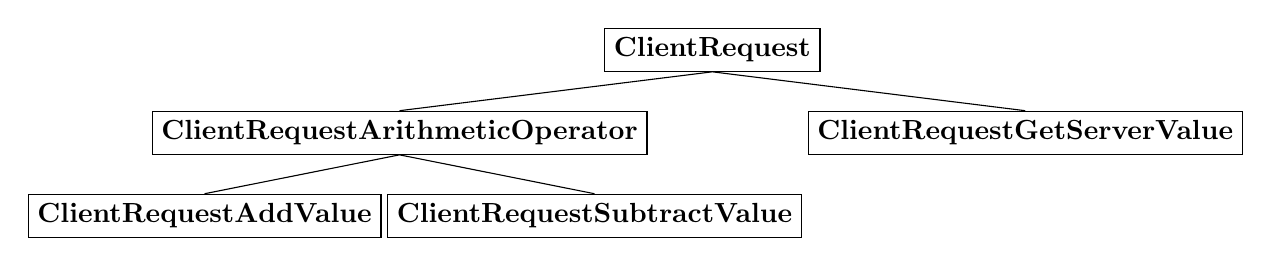
\begin{tikzpicture}[every tree node/.style = draw]
\Tree [.{ {\bfseries ClientRequest} }
	[.{ {\bfseries ClientRequestArithmeticOperator} } 
		[.{ {\bfseries ClientRequestAddValue} } ]
		[.{ {\bfseries ClientRequestSubtractValue} } ]
]
	[.{\bfseries ClientRequestGetServerValue}
]
]
\end{tikzpicture}
\caption{Simple Client/Server ClientRequest type hierarchy}
\label{fig:scs-cri}
\end{figure}


\begin{figure}[ht]
\lstinputlisting[language=Java,linerange=19-43]{ClientRequest.java}
\caption{ClientRequest (abstract class) of simple Client/Server, based on asynchronous message passing}
\label{fig:scs-clientRequest}
\end{figure}

Figure~\ref{fig:scs-cri} depicts the inheritance hierarchy of {\bfseries ClientRequest}. In figure~\ref{fig:scs-clientRequest}, the abstract top class {\bfseries ClientRequest} is defined. On line 2, a clientId parameter common to all requests to enable identification of what client process request comes from so the response can be sent to the right client. The abstract class\footnote{It is not allowed to create instances directly of an abstract class. There are exceptions to this rule, but that is outside the scope of this course.} defines the method \emph{getClientId()} on line 18-20. On line 22, the abstract method \emph{getOperation()} is defined; this method is defined to return the proper enumeration (defined on line 4). The abstract method \emph{getRequestValue} is valid for all arithmetic operations, it returns the value to add or subtract to the server value. 





\subsection{Synchronous Message Passing}

The synchronous message passing is similar to asynchronous message with the exception that the design must reflect the fact that two processes must meet and exchange values.

\subsection{Rendezvous}

There is a Rendezvous in this API. Due to time limitations, it is not described or used. An updated version of this document will be provided later. 

\section{Application Programming Interfaces}

This API is used to make the semantics of processes as close to the semantics used in \cite{andrews_foundations_2000}. Further, the aim is also to reduce the complexity of the Java API for the course. 

\subsection{AndrewsProcess class}

\begin{table}[ht]
\begin{tabular}{|p{0.5\textwidth}|p{0.5\textwidth}|}
\hline
\hline
{\bfseries Method} & {\bfseries Description}\\
\hline\hline
AndrewsProcess(Runnable runnable) &
Creates an AndrewsProcess object that can be started.\\
\hline
int getAndrewsPid() & Returns the process identity, an integer $\geq 0$
\\
\hline
Runnable getRunnable() & Returns the runnable of the current process \\
\hline
static AndrewsProcess[] andrewsProcessFactory(RunnableSpecification[]) & Creates an array of processes according to the specification of an array of RunnableSpecification \\
\hline
static AndrewsProcess currentAndrewsProcess() & Return the currently executing AndrewsProcess object. \\
\hline
static int currentAndrewsProcessId() & Returns the process identity (an integer) of the currently executing AndrewsProcess object. \\
\hline
static int currentRelativeToTypeAndrewsProcessId() & Returns the relative process identity with respect to the type of the Runnable. It is useful to get an identity for handling a particular type of processes.\\
\hline
static void startAndrewsProcesses(AndrewsProcess[]) & Starts the processes\\
\hline
static void uninterruptibleMinimumDelay(int millis)& Delays the process in an uninterruptible way for \emph{millis} time except for terminations causing the entire program to terminate. \\
\hline
\end{tabular}
\caption{AndrewsProcess API subset}
\label{tab:andrewsProcessAPI}
\end{table}

The {\bfseries AndrewsProcess} API is a limiting class that extends {\bfseries Thread} in Java. Most notably, the AndrewsProcess enforces the use of {\bfseries Runnable} and use integers as process identifiers to relates to the semantics used in the examples \cite{andrews_foundations_2000}. The recommended part of the {\bfseries AndrewsProcess} class is found in table~\ref{tab:andrewsProcessAPI}~on~page~\pageref{tab:andrewsProcessAPI}. 

\subsection{Chan class}

\begin{figure}[ht]
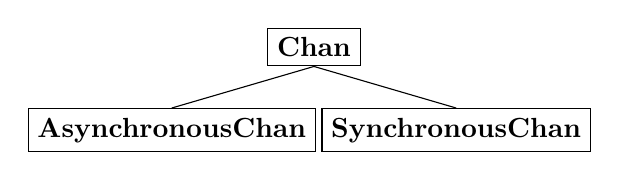
\begin{tikzpicture}[every tree node/.style = draw]
\Tree [.{ {\bfseries Chan} }
	[.{ {\bfseries AsynchronousChan} } 
]
	[.{\bfseries SynchronousChan}
]
]
\end{tikzpicture}
\caption{Chan class hierarchy}
\label{fig:chanHierarchy}

\end{figure}

The {\bfseries Chan} class hierarchy is depicted in figure~\ref{fig:chanHierarchy}~on~page~\pageref{fig:chanHierarchy}. The class {\bfseries Chan} itself is an abstract top class defining the methods \emph{send()} and \emph{receive()}. The {\bfseries AsynchronousChan} is an implementation of the asynchronous message passing and {\bfseries  SynchronousMessagePassing} is an imlplementation of the synchronous message passing. The actual implementation of {\bfseries AsynchronousChan} is based on {\bfseries LinkedBlockingQueue} that closely resembles the semantics of asynchronous message passing with one minor difference. When there is no more space in the queue, an exception is raised in {\bfseries LinkedBlockingQueue}. In contrast, the semantics advocated by Andrews is that \emph{send()} blocks until there is space in the buffer for another message. This latter semantics is implemented in {\bfseries ASynchronousChan}. 

The Chan queues can take any kind of objects of a specified type. This is detemined in the declaration of the variable. For example, \emph{Chan$<$Integer$>$ integerChan=new AsynchronousChan$<$Integer$>$();} creates a channel that can contain integers.

\section{How To Guide}

\subsection{Define a Process}
First you need to create a class that implements the {\bfseries Runnable} interface. Secondly, you need to create processes executing the {\bfseries Runnable} objects.

In figure~\ref{fig:pcsbproc} on page~\pageref{fig:pcsbproc}, a Runnable is defined. The \emph{run()} method overrides the default (abstract) method in the interface. In this particular case, it is a simulated producer process.

 Create an array of {\bfseries RunnableSpecification} and assign each element to an object of {\bfseries RunnableSpecification}. For example, lines 10-12 in figure~\ref{fig:pcsbgps}~on~page~\pageref{fig:pcsbgps}, the array of {\bfseries RunnableSpecification} contains the declaration of 10 producer and 20 consumer processes.  This specification is sent to the factory method on line 17, which returns an array of processes. 

\subsection{Start a Process}
To start a set of processes, take the array of AndrewsProcess objects and pass it to the method that starts all processes. See line 15 in figure~\ref{fig:pcsbgps}.

\subsection{Keep Track of Data Concerning a Process}

Since the process identity, both the global with respect to the application scope and the identity relative to the same type, is an integer, arrays can be employed to keep track of data regarding the processes themselves. For example, in the simple client/server example in section~\ref{sec:simpleClientServer} on page~\pageref{sec:simpleClientServer}, the relative identity of clients are employed to find the channel to send back messages to the client. 

\subsection{Synchronize Processes}

Depends on the mechanism. 

\subsection{Communicate between Processes}

If shared variables are used, then use shared variables. Otherwise, use message passing. 

\subsection{Initialize a Program}
In the class GlobalProgramState, add a public static declaration for each global variable in the solution. Initialized these in the beginning of the \emph{main(String argv)} method. Each process can be initialized in the beginning of the \emph{run()} method. 



\bibliographystyle{apalike}
\bibliography{references}

\end{document}
